\section{Cerința problemei}
Am ales să implementam două tipuri de domenii, unul cu aplicabilitate în lumea reala, și unul fără.
Fiecare domeniu are ca scop realizarea unei rețete. Astfel, prima problemă are ca și scop final realizarea unei prăjituri cu măr, iar cea de a doua are ca scop realizarea unei pizza.

Realizarea unei rețete necesită urmarea unor pași cum ar fi: cumpărarea ingredientelor necesare, realizarea compoziției.

 Problemele definite de domeniul cu aplicabilitate în lumea reală prezintă o stare inițiala parțial definită, acțiunile având efecte nedeterministe, și anume nu știm dacă un anume ingredient e stricat sau nu, urmând ca programul să determine care ingredient e stricat și care nu.
 
 \newline
 Problemele fără aplicabilitate în lumea reală nu întâlnesc aceste situații ale  mediului parțial observabil, aici fiind foarte clar care ingrediente sunt stricate și care nu.
 
 
\newline





\begin{center}
\begin{figure}[htb]
 \centering 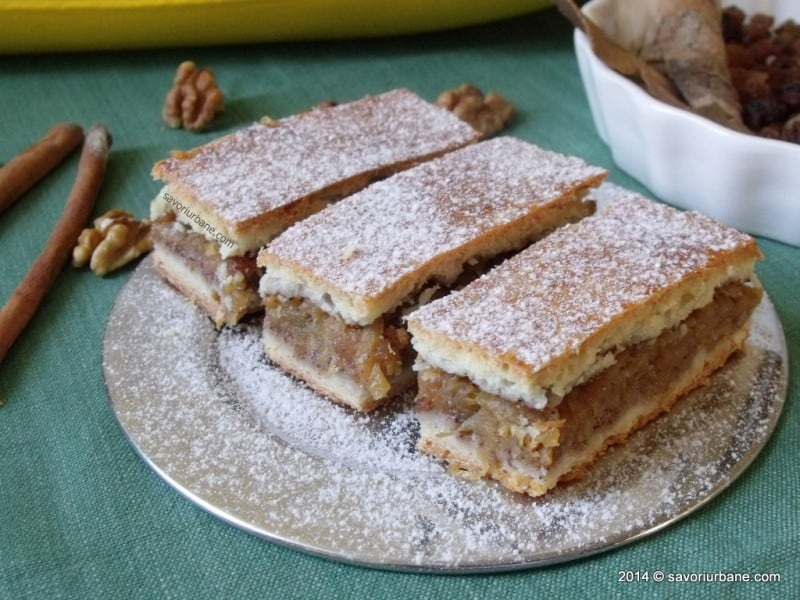
\includegraphics[width=50mm,scale=0.5]{prajitura.jpeg}
 \caption{Goal-ul pentru problema 1.}
  \label{fig:boat1}
  \end{figure}
\end {center}
\begin{figure}[htb]
 \centering 
\includegraphics[width=50mm,scale=0.5]{pizza.jpeg}
 \caption{Goal-ul pentru problema 2.}
  \label{fig:boat2}
  \end{figure}


\newpage